\documentclass{beamer}
\usepackage{circuitikz}
\usepackage{graphicx}
\usepackage{caption}
\usepackage{subcaption}
\usepackage{chngcntr}
\usepackage[customcolors]{hf-tikz}
\usefonttheme{serif}
\setbeamertemplate{caption}[numbered]

\title{$\boxed{\mathbf{ANALISI \ DI \ UN \ FILTRO \ CROSSOVER}}$}
\author{Samuele Lanzi mat. 941813}
\date{7 Aprile, 5 Maggio, 26 Maggio 2021}

\begin{document}

\begin{frame}
    \maketitle
\end{frame}

\begin{frame}{$\mathbf{\ Introduzione}$}
    Il filtro crossover è un tipo di circuito utilizzato nei sistemi di riproduzione audio
allo scopo di dividere il segnale in due range di frequenze associati a due speakers: 
\textit{tweeter} per alte frequenze e \textit{woofer} per basse frequenze.
    \begin{figure}
        \scalebox{.5}{\begin{circuitikz} [scale = 1.7]
\draw 
    (0,0) node[ground] {}
    (0,1)     to [sV, l=$\varepsilon$, fill=yellow] (0, 2)
    (0,2)     to [/tikz/circuitikz/bipoles/length = 20pt, R, l = $R_{\varepsilon}$] (0, 3)
    (0,0.5)   to [short, l_ = AI$0_{-}$, -o] (-1, 0.5)
    (0,3.5)   to [short, l_ = AI$0_{+}$, -o] (-1, 3.5)
    (0,0)     to [short, *-] (0, 1)
    (0,3)     -- (0,4)
    (1.8, 3)  to [L, l_=$L$] (1.8,1.8)
    (1.8,3)   to [/tikz/circuitikz/bipoles/length=20pt, R, l=$R_{IL}$] (1.8,4)
    (1.8, 0)  to [R, l=$R_L$ ] (1.8,1.8)
    (4, 0)    to [R, l=$R_C$ ] (4,1.8)
    (4, 1.8)  to [C, l=$C$ ] (4,3)
    (4,3)     to [/tikz/circuitikz/bipoles/length=20pt, R, l=$R_{IC}$] (4,4)
    (1.8,1.4) to [short, l=AI$1_{+}$,-o] (2.8, 1.4)
    (1.8,0.4) to [short, l=AI$1_{-}$, -o] (2.8, 0.4)
    (4,1.4)   to [short, l=AI$2_{+}$, -o] (5, 1.4)
    (4,0.4)   to [short, l=AI$2_{-}$, -o] (5, 0.4)
    (0, 0)    -- (4, 0)
    (0, 4)    -- (4, 4);

\draw[red,thick,dashed] (-0.6, 1)  to [short, l = $ FGEN $] (-0.6, 3)
                        (-0.6, 3)  -- (0.6, 3)
                        (0.6, 1)   -- (0.6, 3)
                        (-0.6, 1)  -- (0.6, 1);

\draw[green,thick,dashed] (1.2, 2)    -- (1.2, 3.85)
                          (1.2, 3.85) -- (2.4, 3.85)
                          (2.4, 2)    -- (2.4, 3.85)
                          (1.2, 2)    -- (2.4, 2);

\draw[blue,thick,dashed] (3.4, 2)    -- (3.4, 3.85)
                         (3.4, 3.85) -- (4.6, 3.85)
                         (4.6, 2)    -- (4.6, 3.85)
                         (3.4, 2)    -- (4.6, 2);
\end{circuitikz}}
        \caption{\textit{Schema del circuito realizzato}}
    \end{figure}
\end{frame}

\begin{frame}
    La frequenza di separazione del 
segnale è specifica del circuito e viene detta \textit{frequenza di crossover} e si dimostra  che tale frequenza è determinata da:
%%%%%%%%%%%%%%%%%%%%%%%% Equation 1
\hfsetfillcolor{blue!10}
\hfsetbordercolor{blue}
\begin{equation}
    \begin{split}
    \tikzmarkin{d}(0.2,-0.7)(-0.2,0.7)
        \nu_0=\frac{1}{2\pi\sqrt{LC}}=\frac{1}{2\pi\sqrt{\tau_L\tau_C}}
    \tikzmarkend{d}
    \end{split}
\end{equation}
%%%%%%%%%%%%%%%%%%%%%%%
\begin{itemize}
    \item <1-> $\tau_L = \frac{L}{R_L+R_{IL}}$ tempo caratteristico filtro passa-basso;
    \item <2-> $\tau_C= C \ (R_C+R_{IC})$ tempo caratteristico filtro passa-alto;
    \item <3-> La frequenza di crossover attesa calcolata grazie all'equazione (1) ha valore \color{blue}{$\nu_0=(4021 \pm 40) \ Hz$}.
\end{itemize}
\end{frame}

\begin{frame}{$\mathbf{\  Apparato \ Sperimentale}$}
    \begin{itemize}
        \item <1-> Il circuito è stato assemblato sulla breadboard di ELVIS;
        \item <2-> Dapprima sono stati misurati i valori delle componenti tramite il \textit{Digital Multimeter};
        \item <3-> Sono stati acquisiti dati relativi alla tensione in ingresso FGEN e le tensioni ai capi di $R_L$ ed $R_C$;
        \item <4-> Lo \textit{Sweep} è stato eseguito nel range $1 \ kHz - 10 \ kHz$ con incrementi di $10 \ Hz$;
        \item <5-> L'acquisizione è stata effettuata ad una frequenza di campionamento pari a $F_S = 200 \ kHz$;
        \item <6-> L'ampiezza e la fase sono state estrapolate da ogni acquisizione grazie al subVI \textit{Extract Single Tone Information} di LabVIEW. 
    \end{itemize}
\end{frame}

\begin{frame}{$\mathbf{\  Risultati \ e \ Discussione - Analisi \ preliminare}$}
    \begin{figure}
        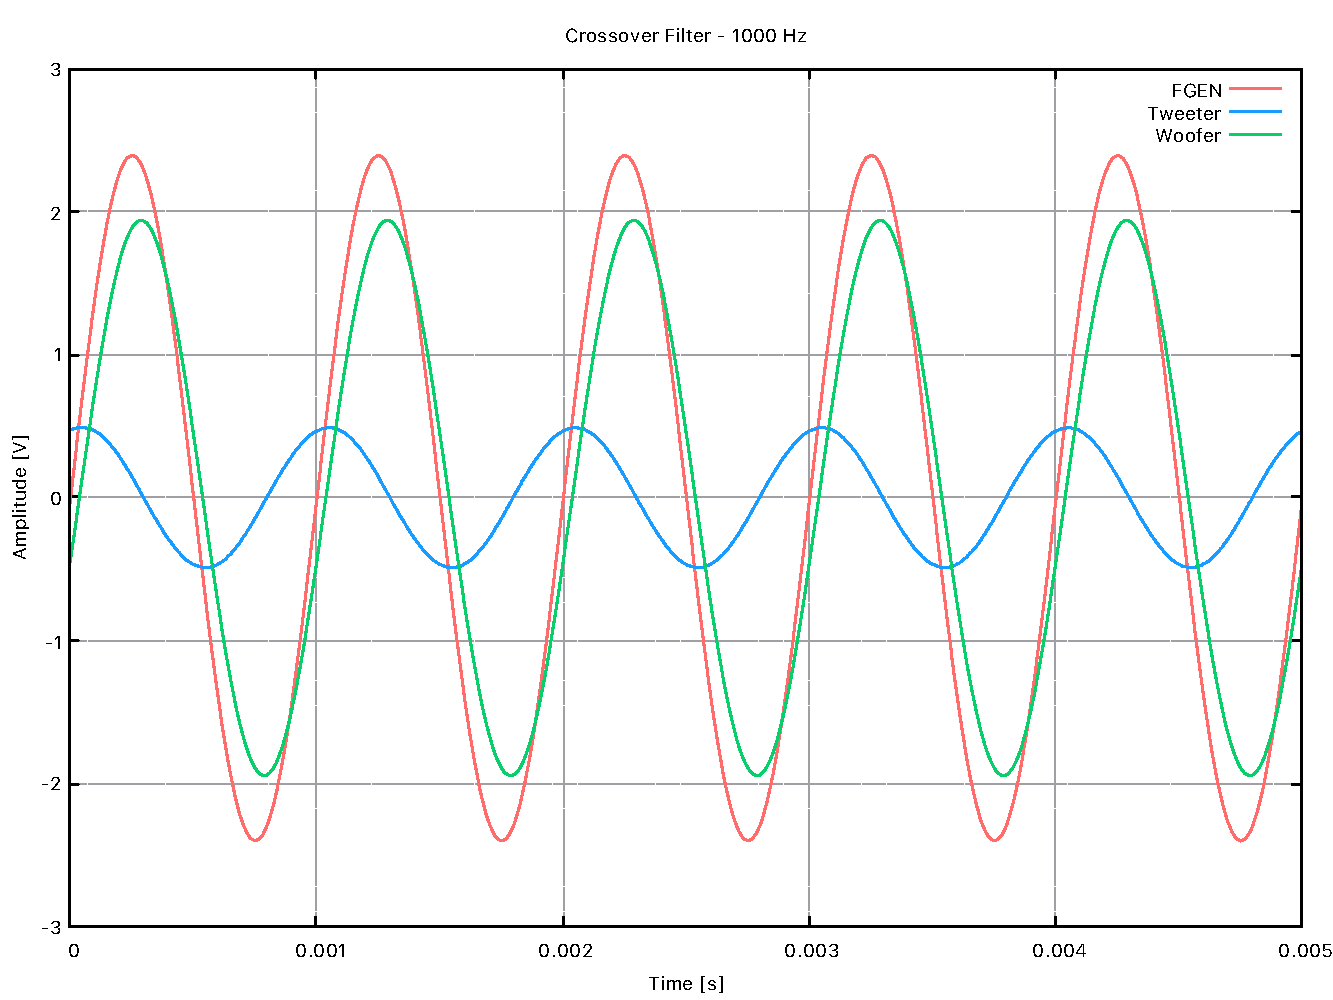
\includegraphics[width=0.45\linewidth]{../results/CF1000Hz.pdf}
        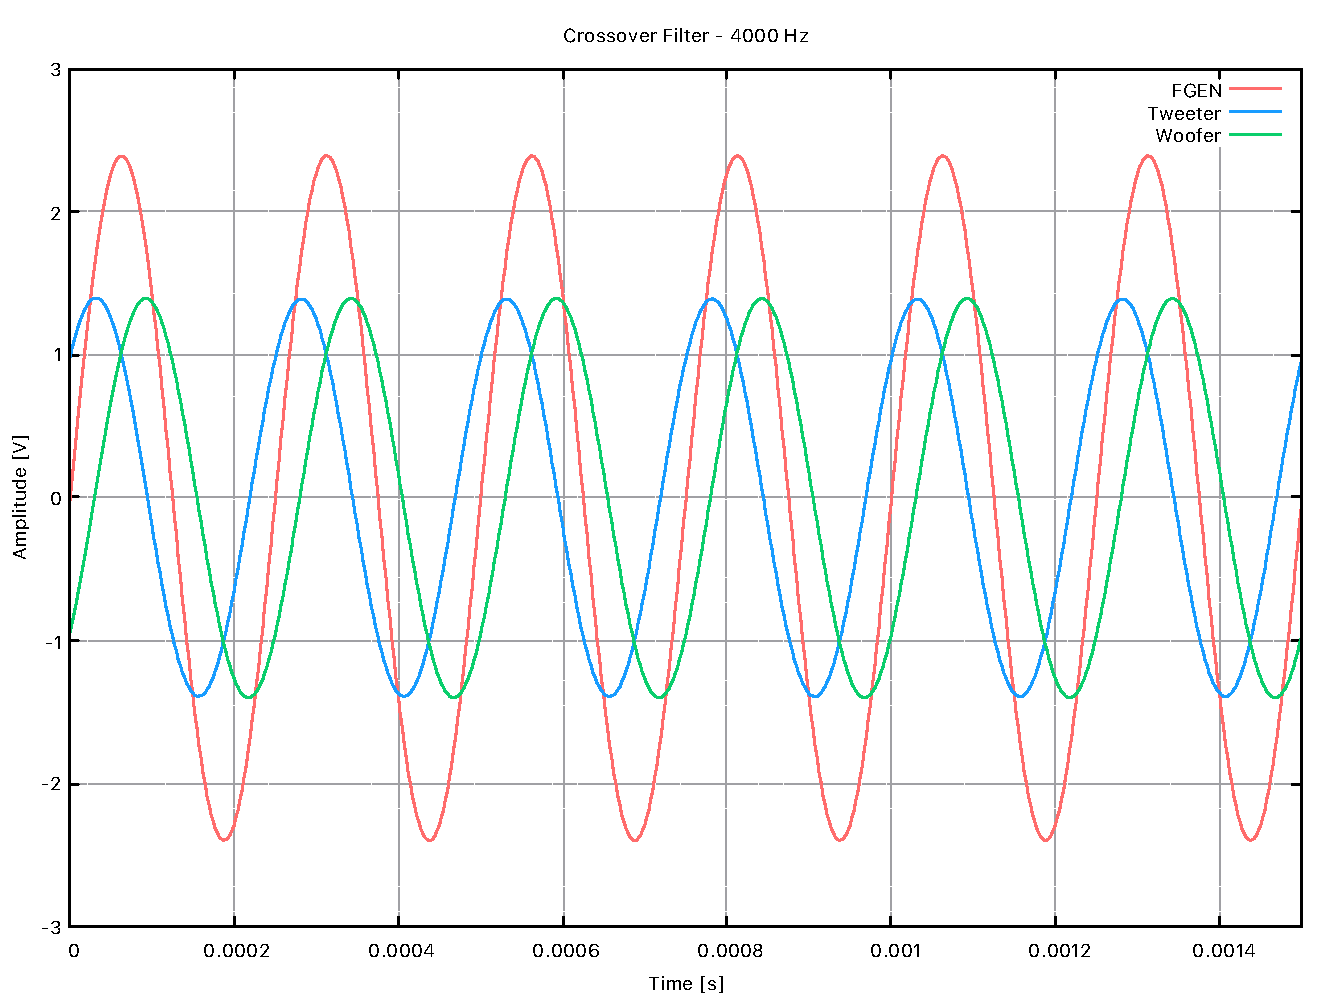
\includegraphics[width=0.45\linewidth]{../results/CF4000Hz.pdf}
        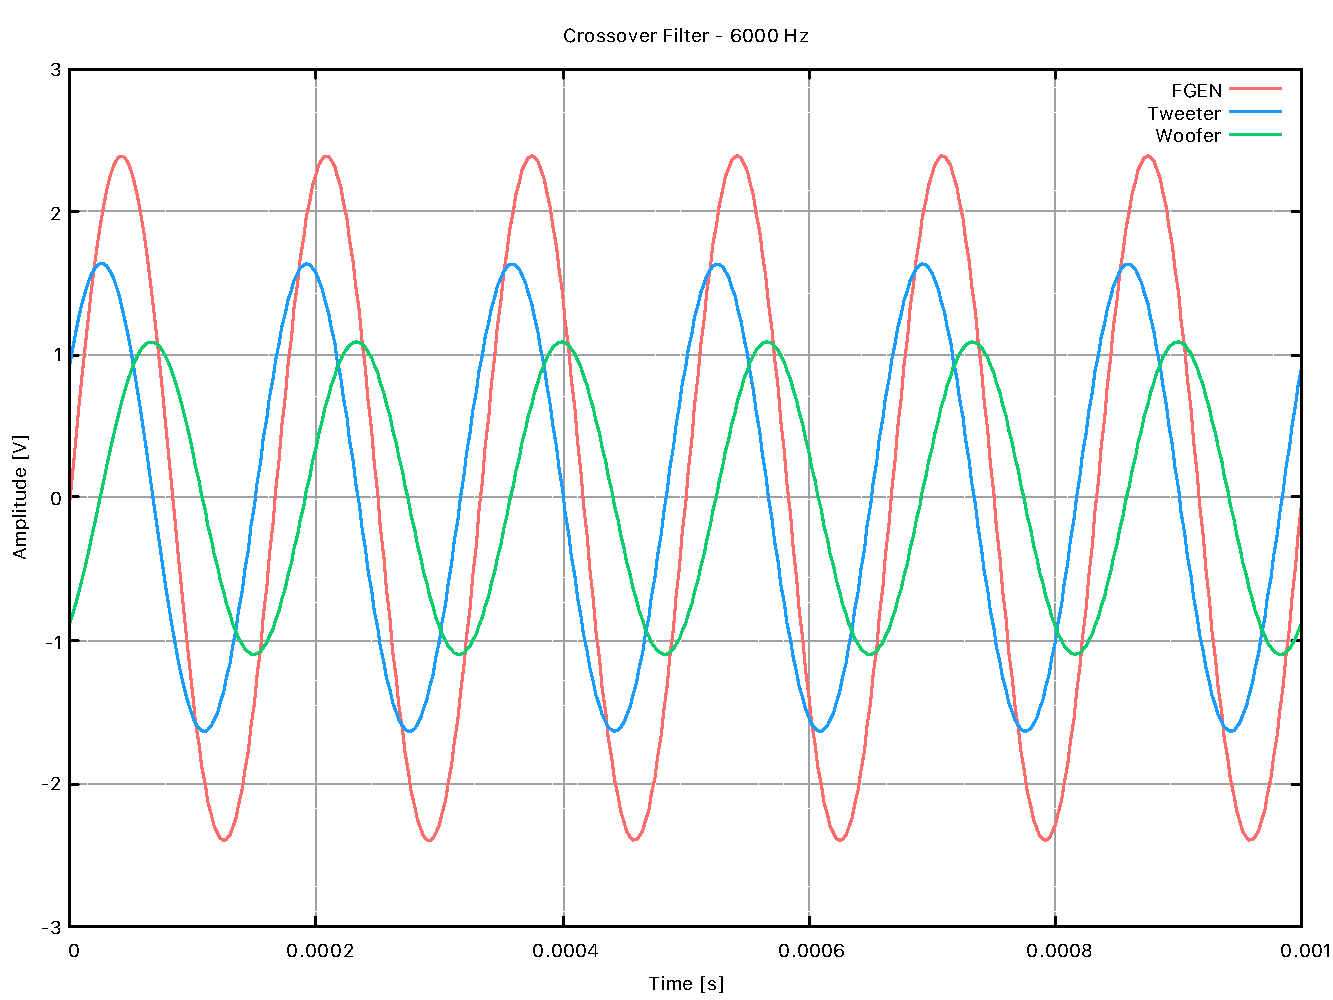
\includegraphics[width=0.45\linewidth]{../results/CF6000Hz.pdf}
        \caption{\textit{Analisi preliminare del circuito: Segnale sinusoidale.}}
    \end{figure}
\end{frame}

\begin{frame}
    Effetti del filtro sui vari segnali in entrata. I dati sono rappresentati da linee continue a causa dei numerosi punti ravvicinati.
    \begin{figure}
        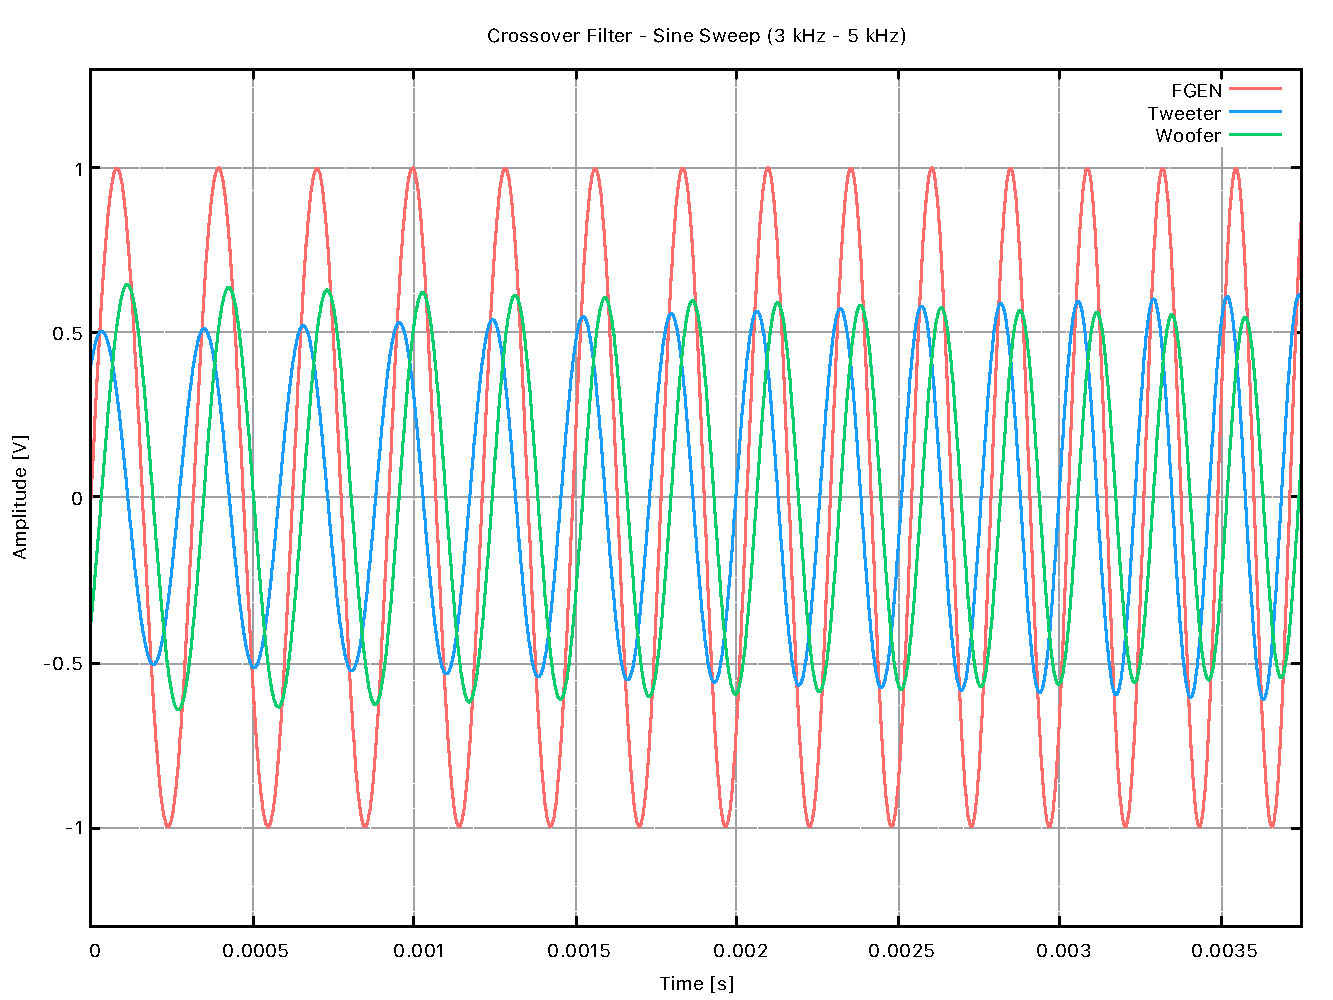
\includegraphics[width=0.45\linewidth]{../results/CFSineSweep.pdf}
        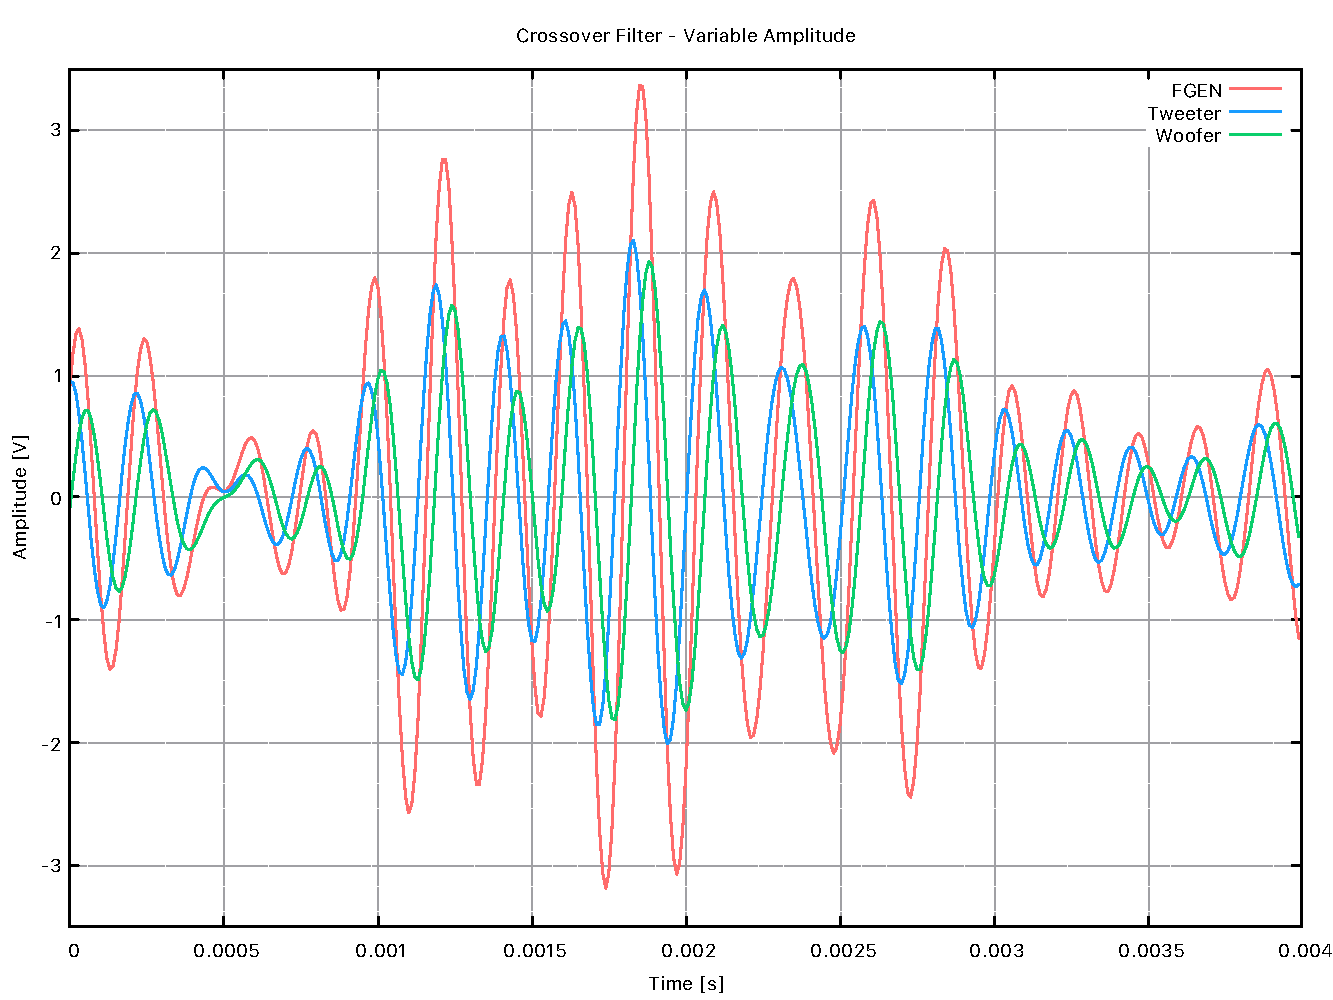
\includegraphics[width=0.45\linewidth]{../results/CFAmplitudeMod.pdf}
        \caption{\textit{Analisi preliminare del circuito: Arbitrary Waveform.}}
    \end{figure}
\end{frame}

\begin{frame}{$\mathbf{\ Risultati \ e \ Discussione - Analisi \ della \ tensione}$}
    Equazioni che forniscono le curve teoriche della tensione:
    \begin{itemize}
        \item <1-> Per il ramo woofer:
        \begin{equation*}
            \mathbf{V} = (R_{IL}+j\omega L)\mathbf{I}_L + \mathbf{V}_L=\frac{R_{IL}+j\omega L}{R_L+R_{IL}+j\omega L} \mathbf{V} + \mathbf{V}_L
        \end{equation*}
        \begin{equation*}
            \mathbf{V}_L=\frac{R_{IL}}{R_L+R_{IL}+j\omega L} \mathbf{V} =\frac{r_L}{1+j\omega \tau_L} \mathbf{V}
        \end{equation*}
        \hfsetfillcolor{blue!10}
        \hfsetbordercolor{blue}
        \begin{equation}
            \Rightarrow 
            \begin{split}
                \tikzmarkin{b}(0.2,-0.55)(-0.2,0.55)
                    |\mathbf{V}_L(\nu)|= \frac{r_L}{\sqrt{1+(2 \pi \tau_L \nu)^2}}V
                \tikzmarkend{b}
                \end{split}
        \end{equation}
        \item <2-> Analogamente per il ramo del tweeter:
        \hfsetfillcolor{blue!10}
        \hfsetbordercolor{blue}
        \begin{equation}
            \Rightarrow 
            \begin{split}
                \tikzmarkin{c}(0.2,-0.75)(-0.2,0.7)
                    |\mathbf{V}_C(\nu)|= \frac{r_C}{\sqrt{1+\frac{1}{(2 \pi \tau_C \nu)^2}}}V
                \tikzmarkend{c}
            \end{split}
        \end{equation}
    \end{itemize}
\end{frame}
\begin{frame}
    \begin{figure}
        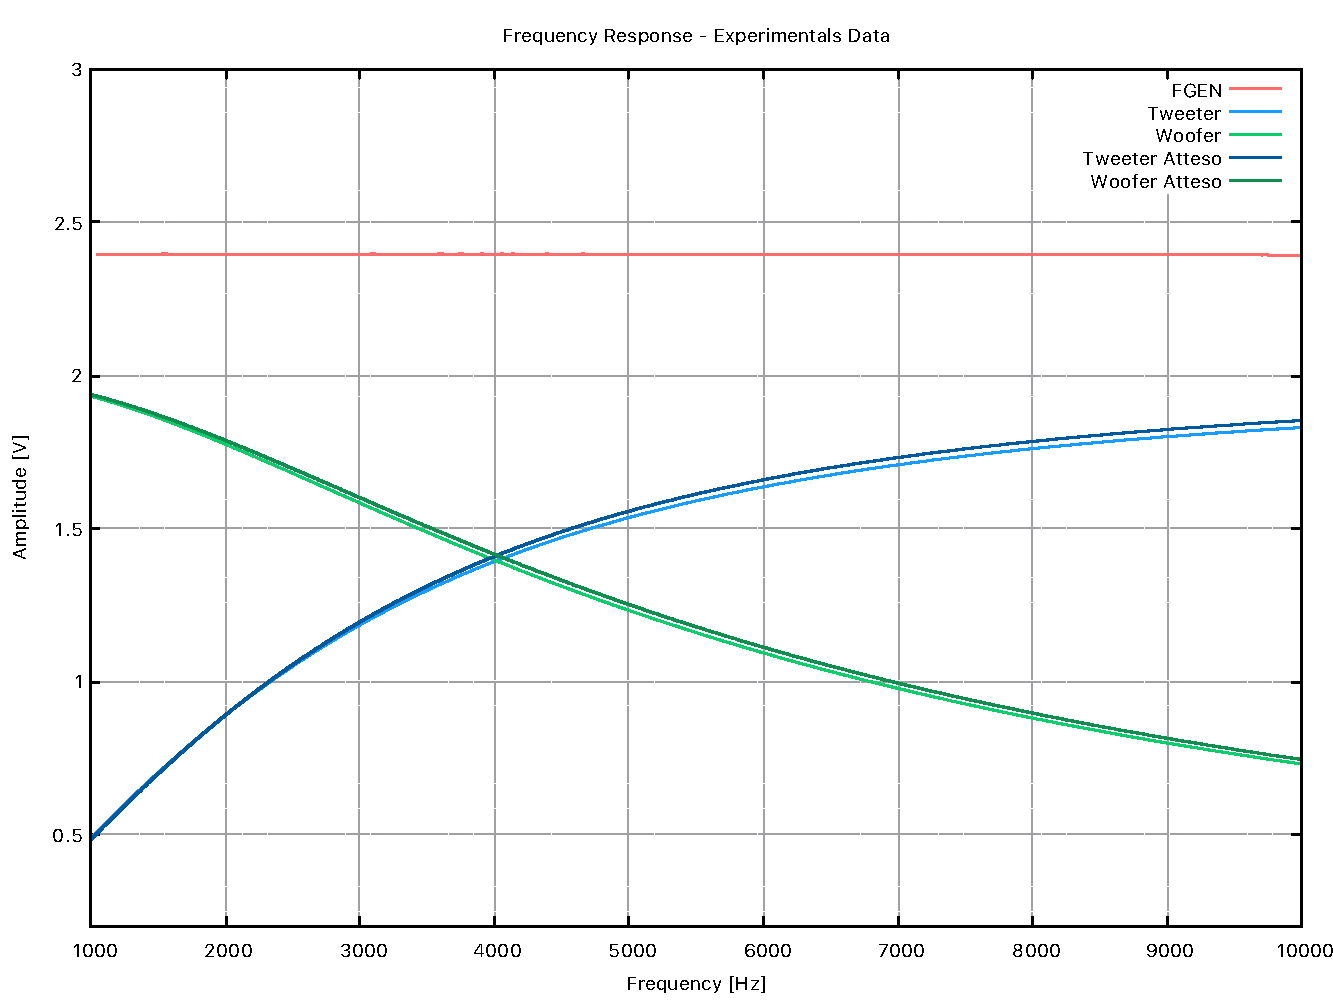
\includegraphics[width=0.45\linewidth]{../results/CFAmpl.pdf}
        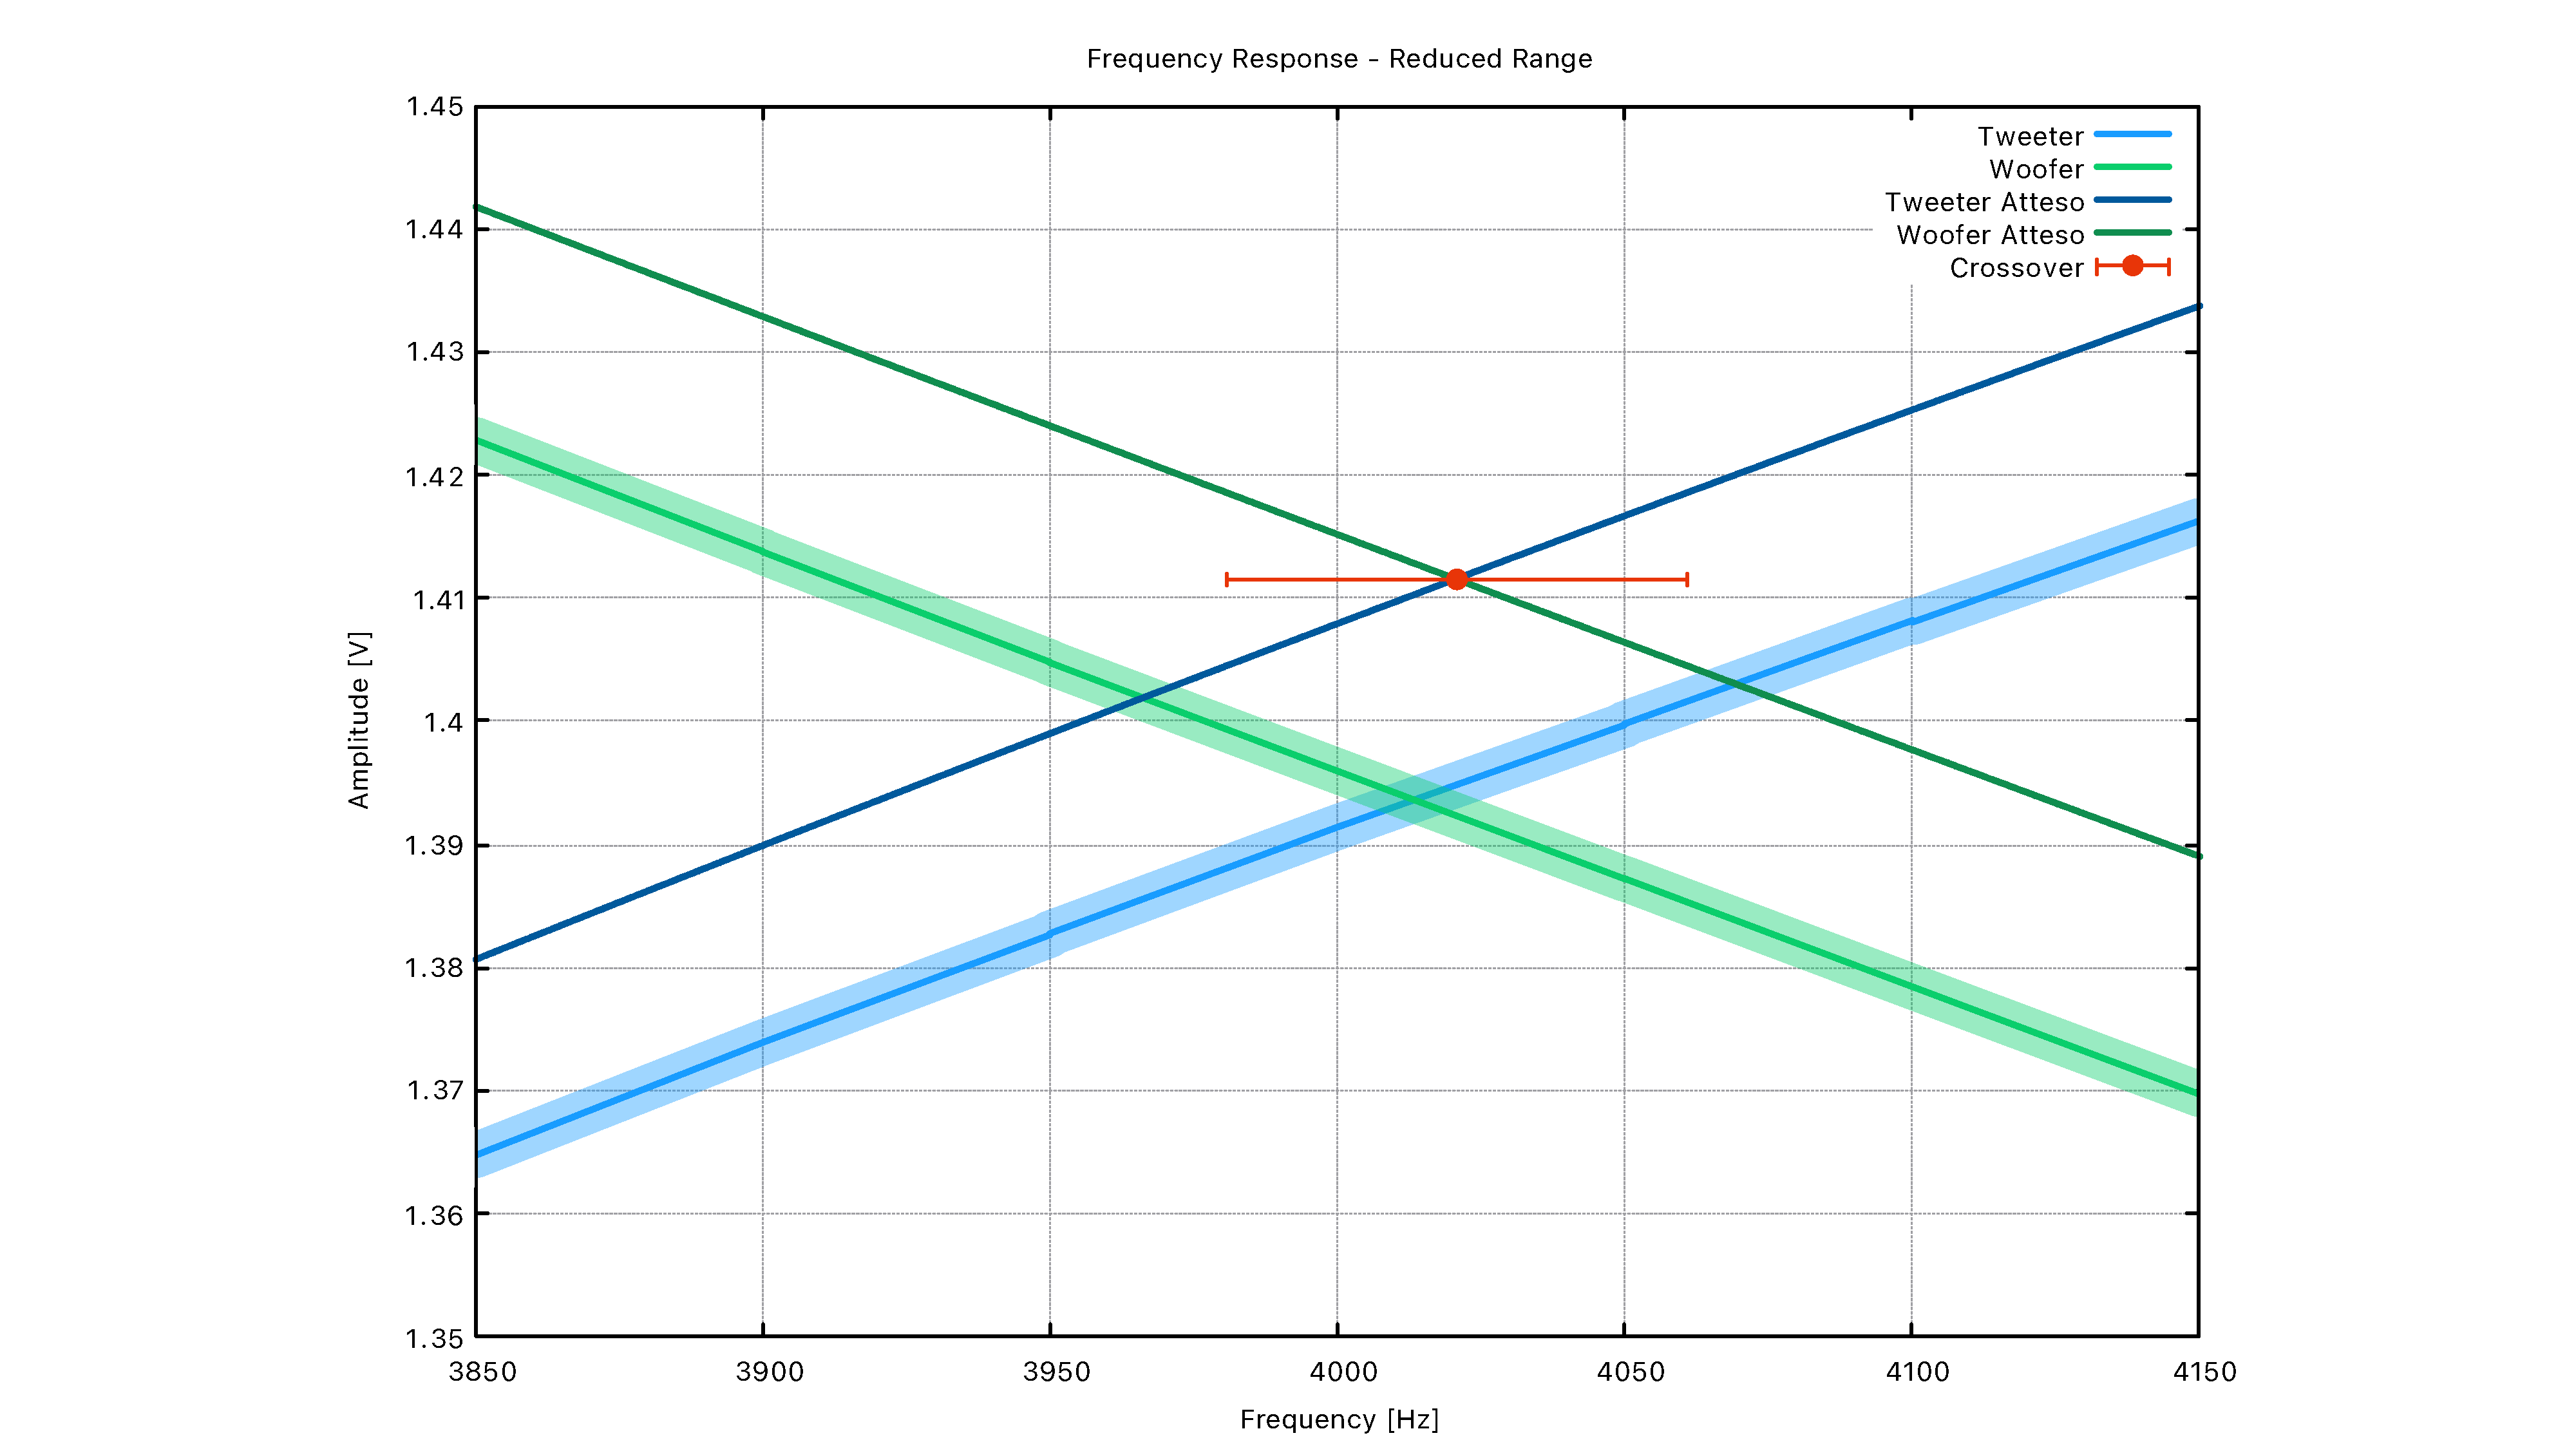
\includegraphics[width=0.45\linewidth]{../results/CFAmplRR.pdf}
        \caption{\textit{Ampiezza del segnale rilevato e funzioni attese.}}
    \end{figure}
    \begin{itemize}
        \item <1-> Ai dati sperimentali è stata associata un'incertezza sull'ampiezza di $\delta V =  2 \ mV$ ;
        \item <2-> Le incertezze sulla frequenza sono confrontabili con la risoluzione del \textit{Function Generator} $\delta \nu = 0.186 \ Hz$, del tutto trascurabili.
        \item <3-> Per costruzione $r_C \approx r_L = (0.83 \pm 0.01) $;
    \end{itemize}
\end{frame}

\begin{frame}
    \begin{itemize}
        \item In Fig. 4 notiamo che la curva FGEN si discosta dal valore atteso di $2.5 V$ in quanto vi è una piccola caduta di potenziale dovuta alla resistenza interna di ELVIS.
    \end{itemize}

    Per determinare la frequenza di crossover a partire dall'analisi dell'ampiezza è stato eseguito il fit delle funzioni in equazione (2) e (3) sui dati sperimentali:
    \begin{figure}
        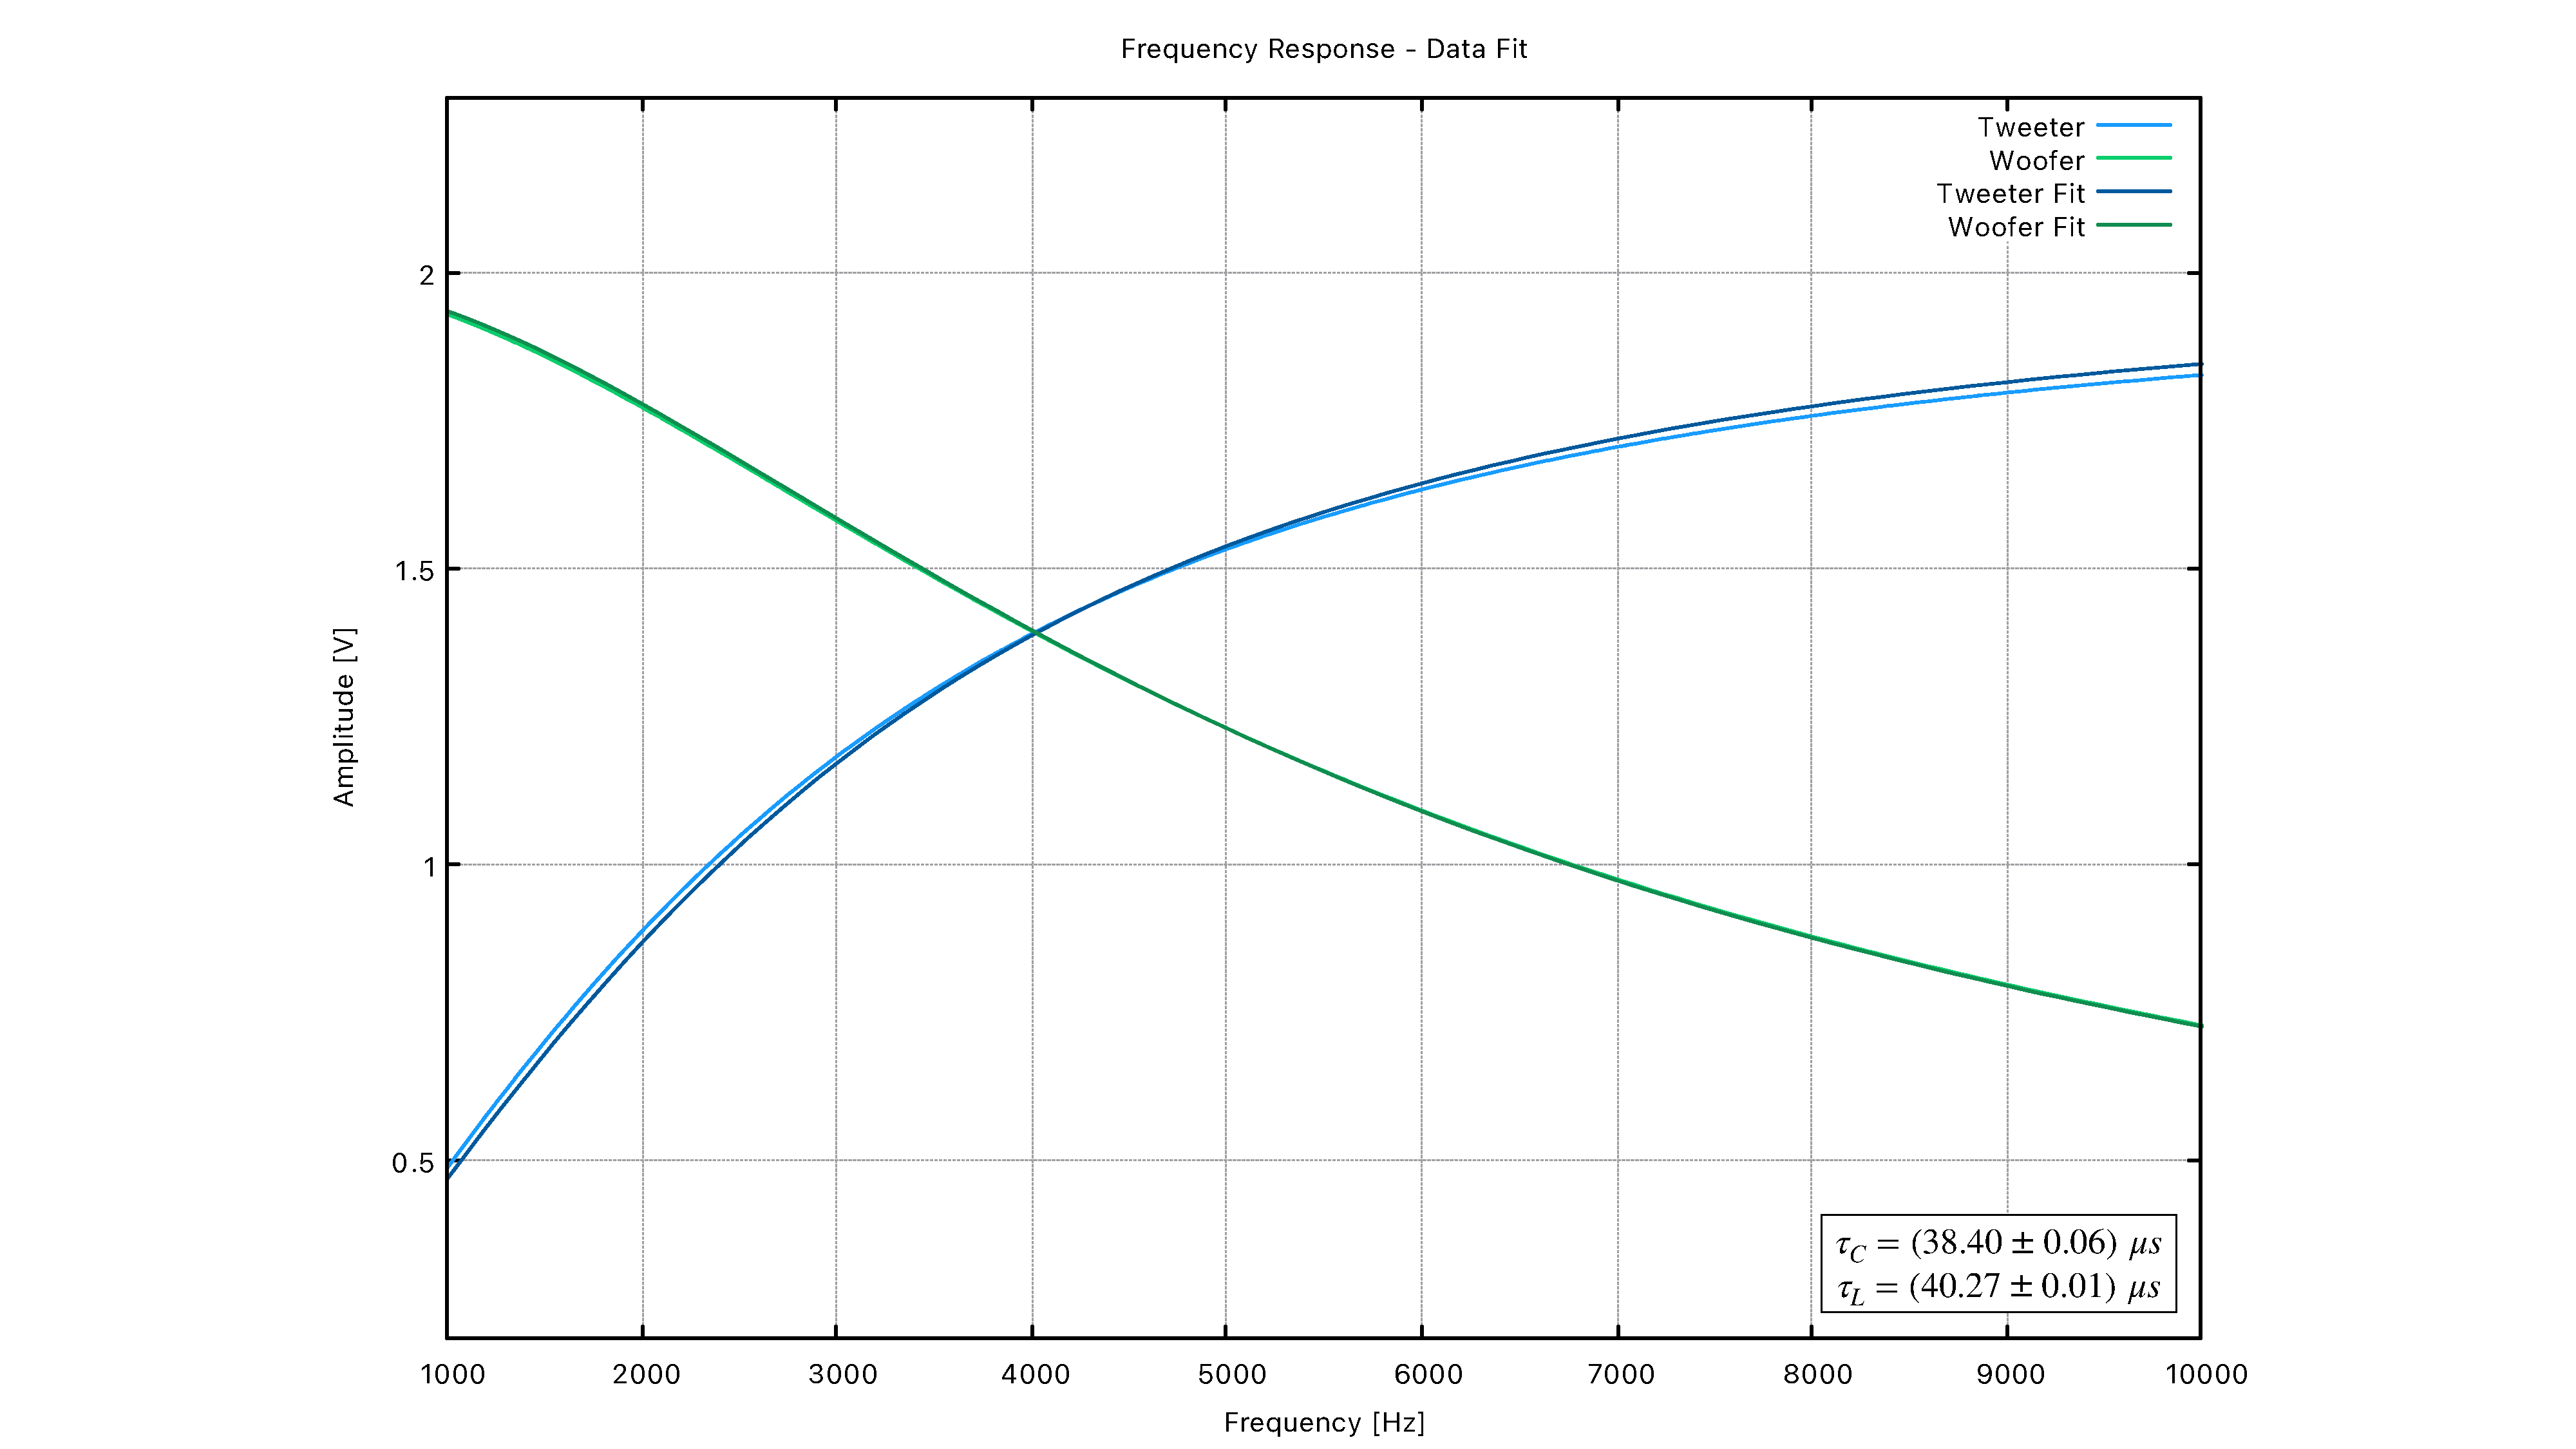
\includegraphics[width=0.45\linewidth]{../results/CFAmplFit.pdf}
        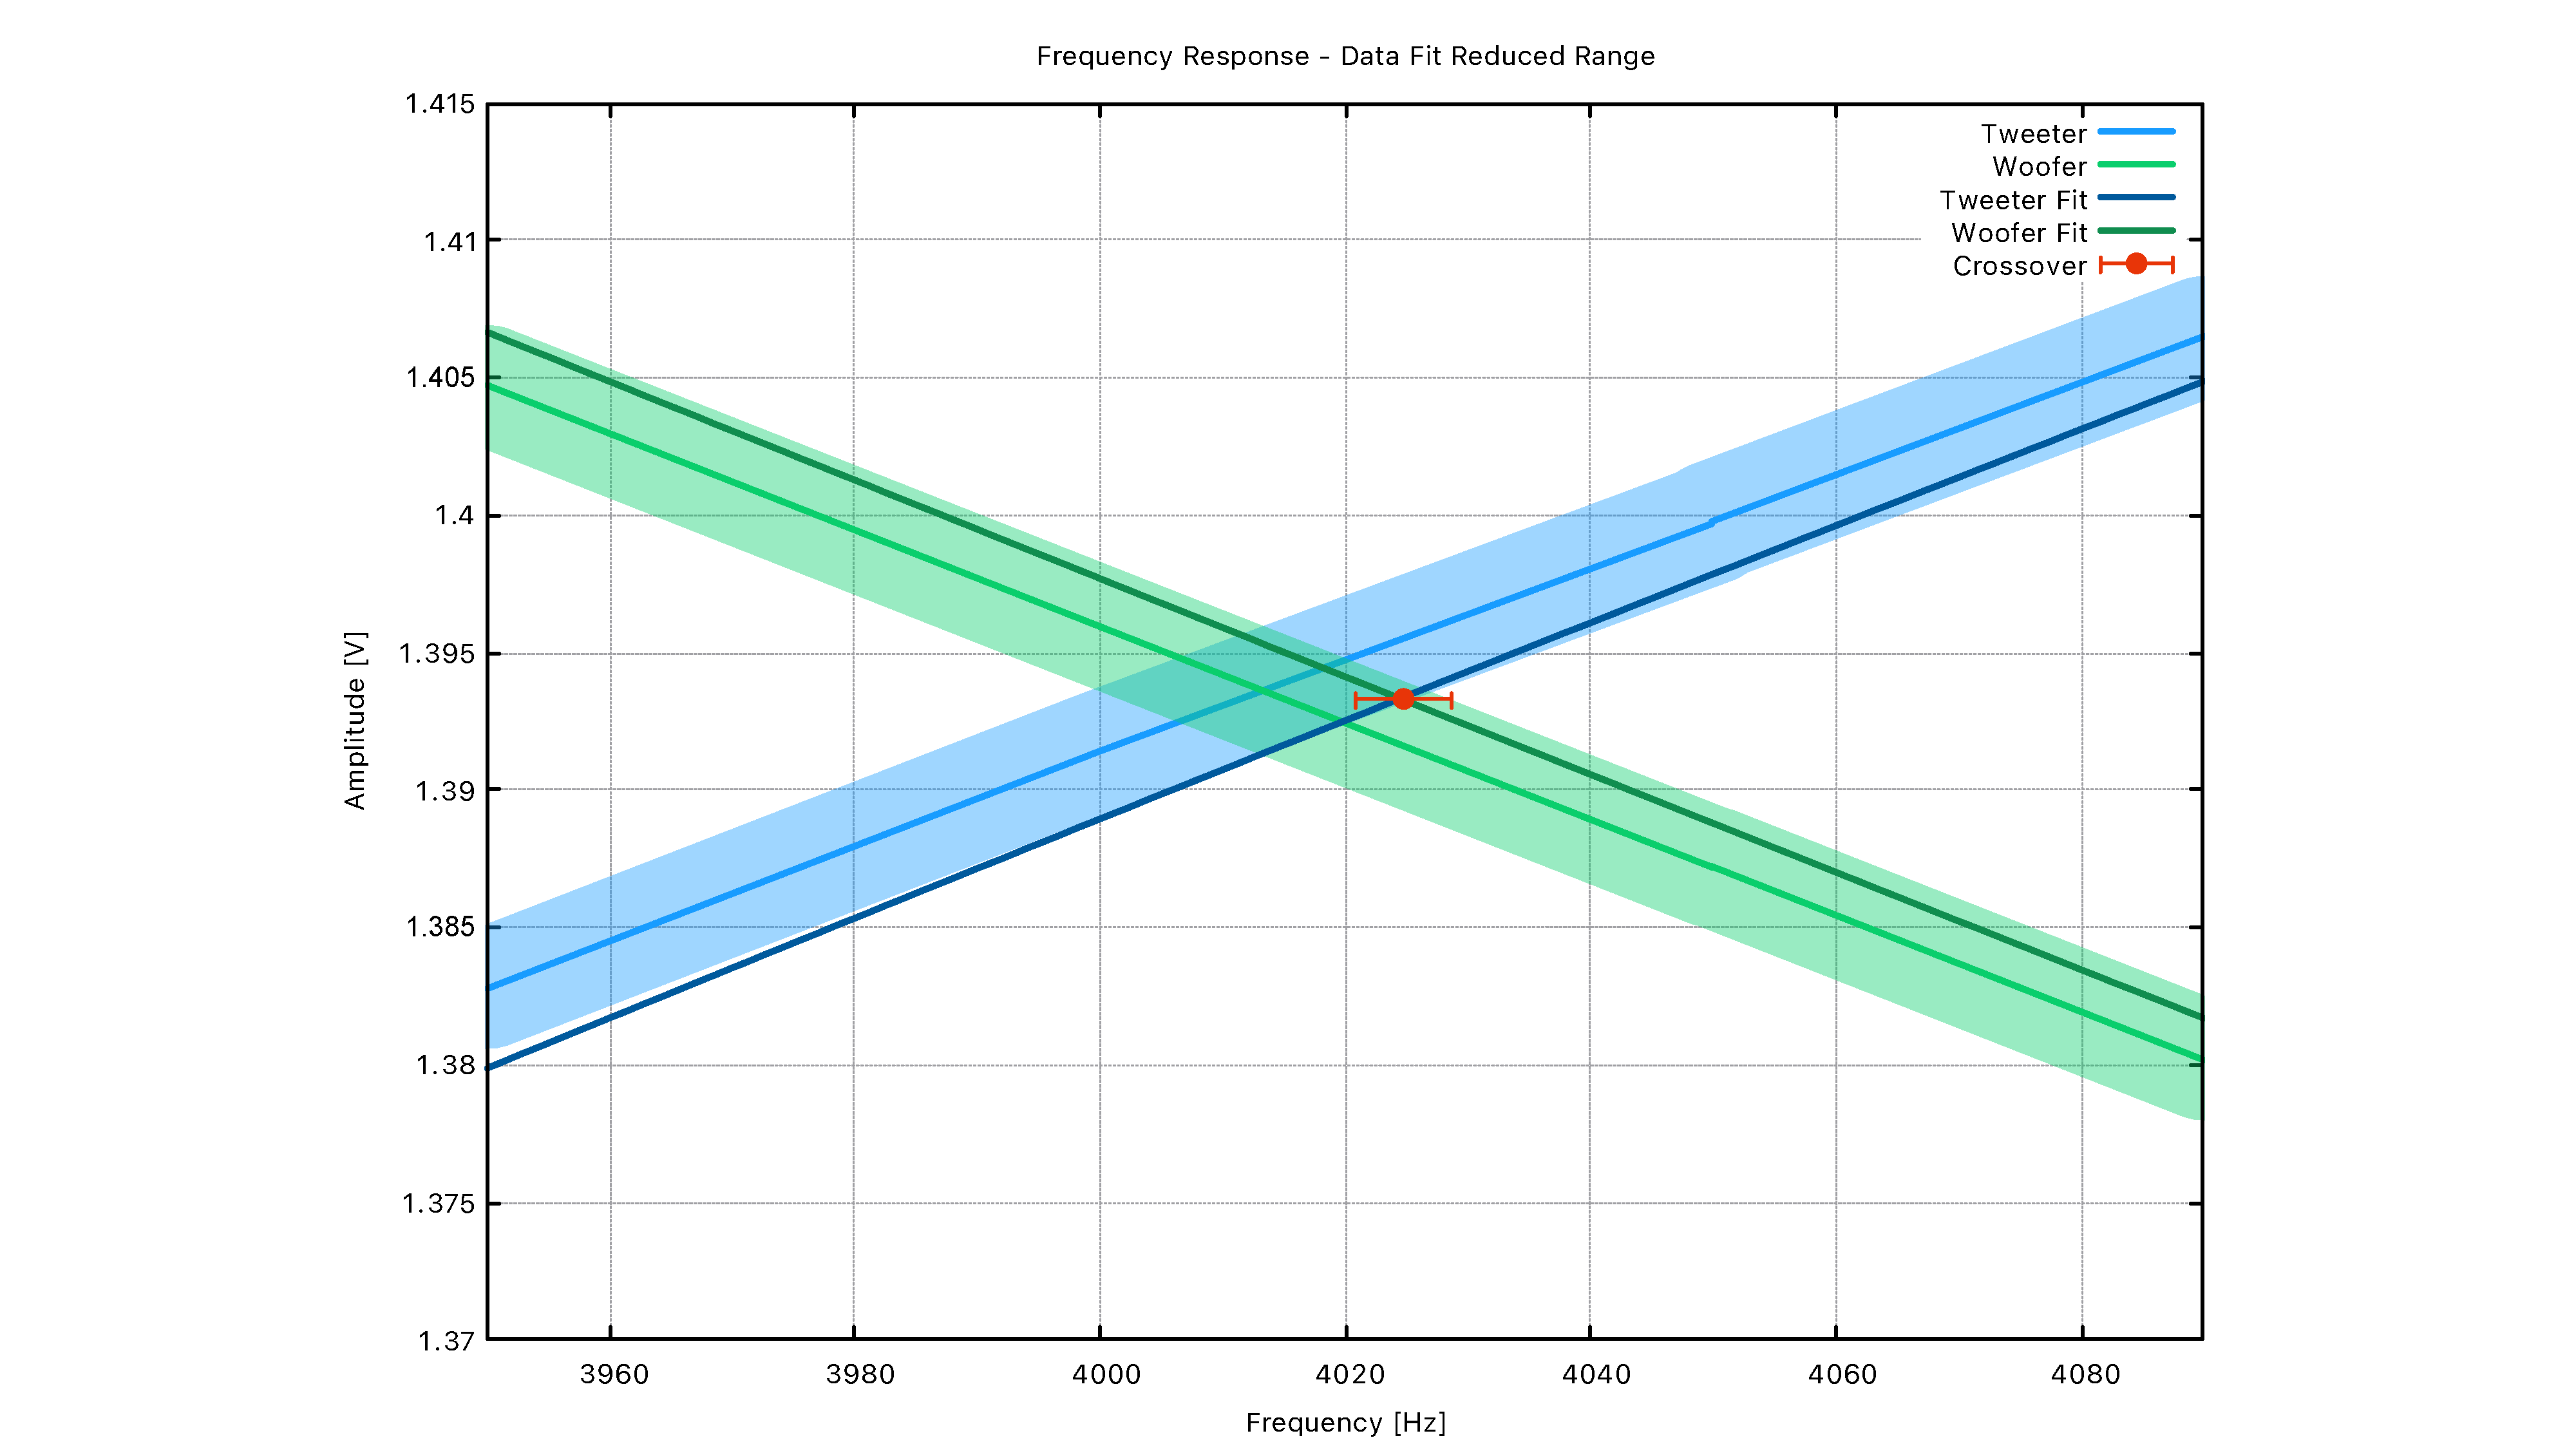
\includegraphics[width=0.45\linewidth]{../results/CFAmplRRFit.pdf}
        \caption{\textit{Fit dati sperimentali.}}
    \end{figure}
\end{frame}

\begin{frame}
    \begin{itemize}
        \item <1-> I valori dei parametri del fit sono risultati essere: $\tau_C = (38.40 \pm 0.06) \ \mu s$ e $\tau_L = (40.27 \pm 0.01) \ \mu s$ 
        molto vicini a quelli attesi $\tau_C=(39.6\pm0.8) \ \mu s $ e $\tau_L=(39.6\pm0.7) \ \mu s $.
        \item <2-> I fit sono stati effettuati considerando FGEN costante $\rightarrow$ è stata considerata un'incertezza pari alla massima distanza tra 
        i dati relativi ad FGEN ed il valor medio, cioè $20 \ mV$;
        \item <3-> A questi fit sono associati i valori di chi quadrato ridotto: $\tilde{\chi}^2_C=0.44$ e $\tilde{\chi}^2_L=0.07$. 
        \item <4-> La miglior stima della frequenza di crossover è risultata essere: \color{blue}{$\nu_0=(4024 \pm 4) \ Hz$}.
    \end{itemize}
\end{frame}

\begin{frame}{$\mathbf{\ Risultati \ e \ Discussione - Analisi \ della \ fase}$}
    Le equazioni che forniscono le curve teoriche della fase sono:
    \begin{itemize}
        \item <1-> Per il tweeter:
    \hfsetfillcolor{blue!10}
    \hfsetbordercolor{blue}
    \begin{equation}
        \tikzmarkin{e}(0.2,-0.7)(-0.2,0.7)
            \phi_C(\nu)= \arctan\bigg( \frac{1}{2 \pi \tau_C \nu}\bigg)
        \tikzmarkend{e} 
    \end{equation}
    \item <2-> per il woofer:
    \hfsetfillcolor{blue!10}
    \hfsetbordercolor{blue}
    \begin{equation}
        \tikzmarkin{f}(0.2,-0.4)(-0.2,0.5)
            \phi_L(\nu)= -\arctan(2 \pi \tau_L \nu)
        \tikzmarkend{f} 
    \end{equation}
    \item [] <3-> \begin{figure}
        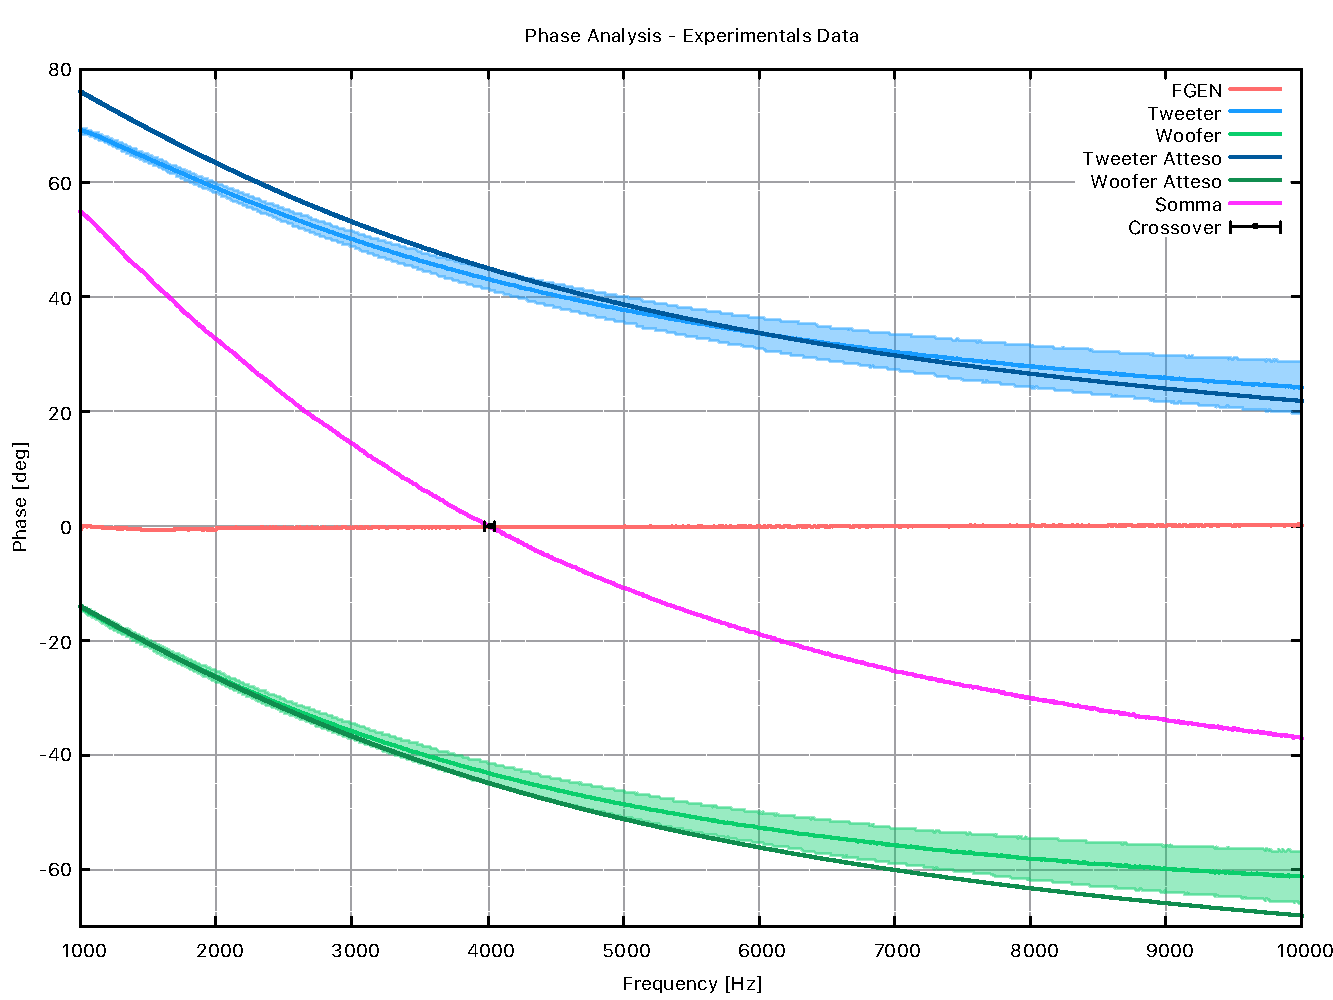
\includegraphics[width=0.45\linewidth]{../results/CFPhase.pdf}
        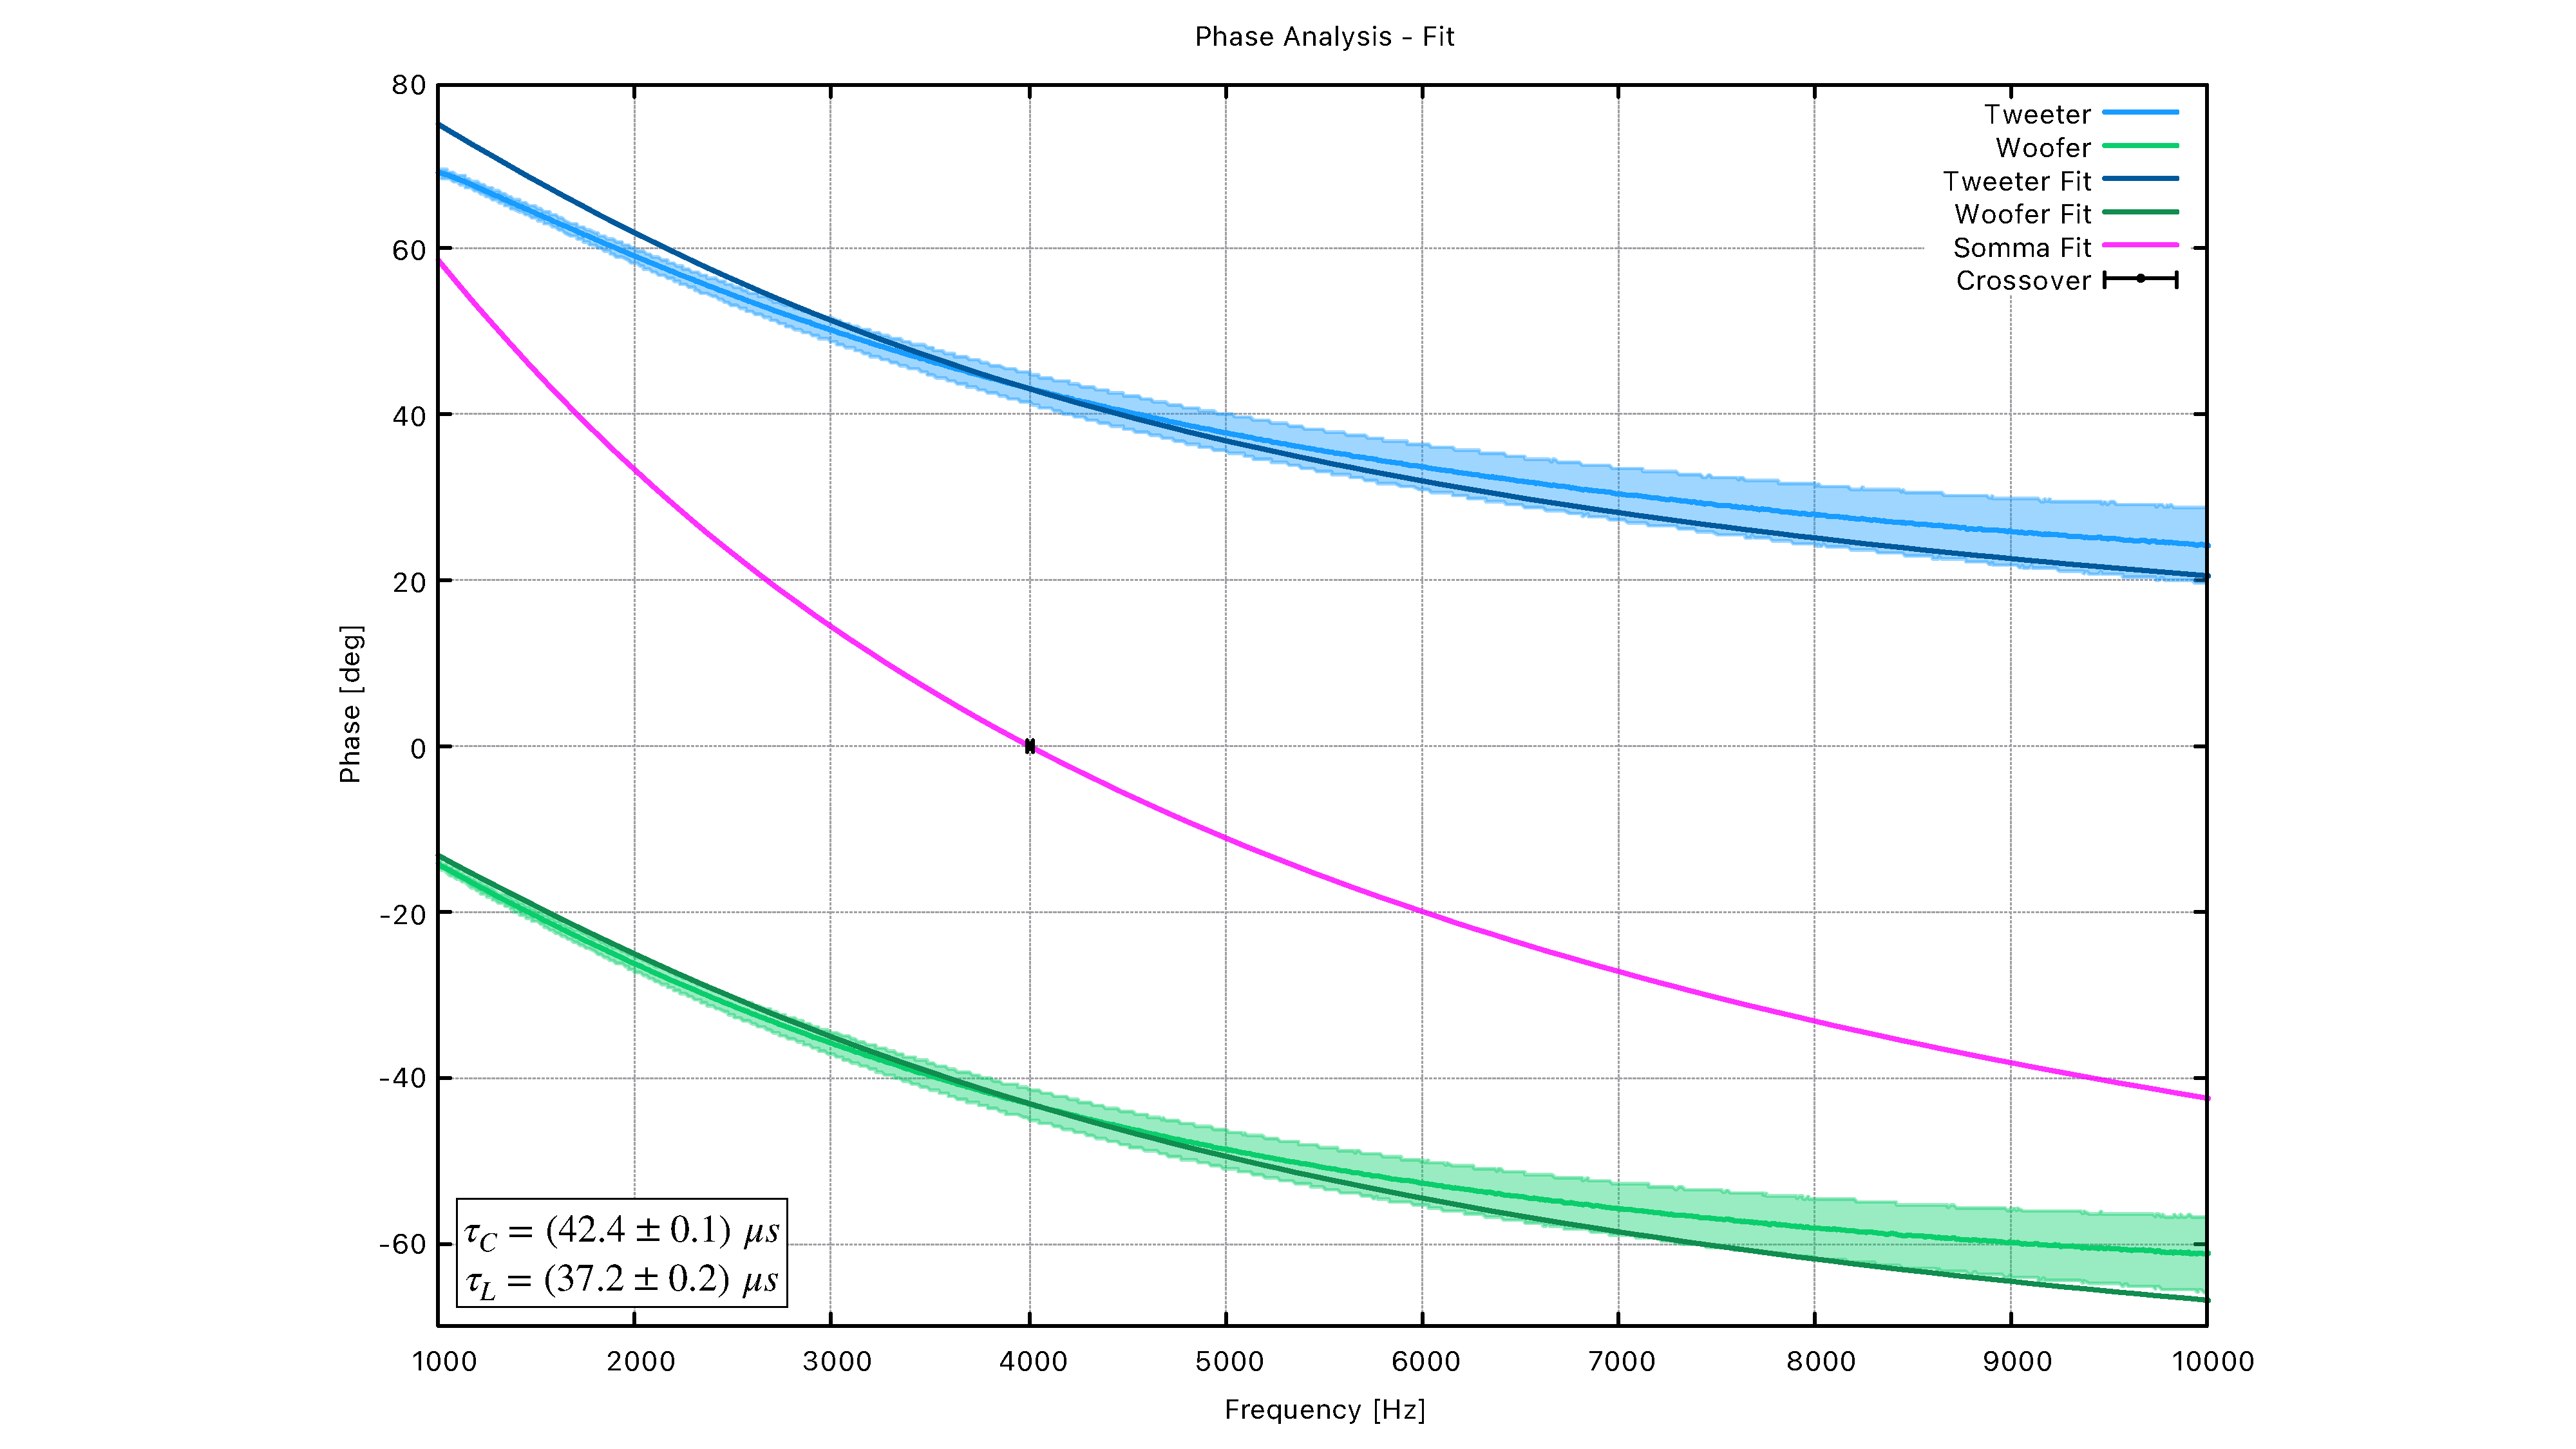
\includegraphics[width=0.45\linewidth]{../results/CFPhaseFit.pdf}
        \caption{\textit{Analisi della fase: dati sperimentali, curve teoriche e fit.}}
    \end{figure} 
    \end{itemize}
\end{frame}

\begin{frame}
    \begin{itemize}
        \item <1-> Ai dati sperimentali è stata associata l'incertezza 
        $\delta \phi = 180 \times \nu / F_S $;
        \item <2-> Il fit delle equazioni (4) e (5) sui dati sperimentali ha fornito i parametri: $\tau_C=(42.41 \pm 0.11) \ \mu s$ e $\tau_L=(37.2 \pm 0.2) \ \mu s$;
        \item <3-> A questi fit sono associati i valori del chi quadrato ridotto $\tilde{\chi}^2_C=1.45$ e $\tilde{\chi}^2_L=0.91$;
        \item <4-> La miglior stima della frequenza di crossover è risultata essere: \color{blue}{$\nu_0=(4007 \pm 16) \ Hz$}.
    \end{itemize}
\end{frame}

\begin{frame}{$\mathbf{\ Conclusione}$}
    \begin{itemize}
        \item <1-> L'analisi dei dati relativi alla tensione ai capi delle resistenze $R_C$ ed $R_L$ ha evidenziato un andamento molto simile a quello previsto e ha portato 
        ad una stima della frequenza di crossover $\nu_0 = (4024 \pm 4) \ Hz$ in accordo con quella attesa.
        \item <2-> L'analisi dello sfasamento è stata altrettanto soddisfacente ed ha evidenziato un andamento simile a ciò che ci si aspettava. La stima della 
        frequenza di crossover è stata $\nu_0 = (4007 \pm 16) \ Hz$.
        \item <3-> Il test d'ipotesi svolto 
        in ambedue le analisi ha portato a valori del chi quadrato ridotto relativamente lontani dal valore ottimale di 1 (soprattutto nell'analisi della tensione). Questa leggera discordanza 
        può essere attribuita ad una stima sbagliata dell'incertezza associata a fase ed ampiezza (probabilmente sovrastimate).
    \end{itemize}
\end{frame}
\end{document}